\documentclass[12pt, a4paper, oneside]{report}

\usepackage[utf8]{inputenc}
\usepackage{geometry}
\usepackage{amsmath, amssymb, amsfonts} % For advanced math
\usepackage{graphicx}   % For including images
\usepackage{hyperref}   % For clickable links/references
\usepackage{listings}   % [FIXED] Correct package name for code snippets
\usepackage{xcolor}     % For color definitions
\usepackage{booktabs}   % For professional tables
\usepackage{titlesec}   % For custom chapter formatting
\usepackage{fancyhdr}   % For headers and footers
\usepackage{appendix}   % For appendix management
\usepackage{float}      % Required for the [H] specifier to force figure placement
\usepackage{tikz}
\usetikzlibrary{shapes.geometric, arrows.meta, positioning, fit, calc, backgrounds, shadows}

% --- Page Geometry ---
\geometry{
    left=30mm,
    right=25mm,
    top=25mm,
    bottom=25mm
}

% --- Code Listing Style ---
\definecolor{codegreen}{rgb}{0,0.6,0}
\definecolor{codegray}{rgb}{0.5,0.5,0.5}
\definecolor{codepurple}{rgb}{0.58,0,0.82}

\lstdefinestyle{mystyle}{
    commentstyle=\color{codegreen},
    keywordstyle=\color{magenta},
    numberstyle=\tiny\color{codegray},
    stringstyle=\color{codepurple},
    basicstyle=\ttfamily\footnotesize,
    breakatwhitespace=false,         
    breaklines=true,                 
    captionpos=b,                    
    keepspaces=true,                 
    numbers=left,                    
    numbersep=5pt,                  
    showspaces=false,                
    showstringspaces=false,
    showtabs=false,                  
    tabsize=2
}
\lstset{style=mystyle}

% --- Header/Footer Setup ---
\pagestyle{fancy}
\fancyhf{}
\fancyhead[L]{\leftmark}
\fancyfoot[C]{\thepage}

% --- Title Data ---
\title{\textbf{ASV Sim Technical Documentation}}

\begin{document}

% --- Title Page ---
\maketitle

% --- Abstract ---
\begin{abstract}
This application presents the design, implementation, and mathematical validation of a control center for an Autonomous Surface Vessel (ASV). The system functions as a Digital Testing Environment (DTE), providing a high-fidelity interface for real-time monitoring, teleoperation, and autonomous trajectory planning. By integrating a First-Order Nomoto model with a Python-based graphical interface and a Robot Operating System 2 (ROS 2) communication backend, the system demonstrates robust capabilities in kinematic simulation and guidance law execution. This document details the system architecture, the derivation of the governing physical equations, and the operational protocols for the end-user.
\end{abstract}

% --- Table of Contents ---
\tableofcontents
\newpage

% =============================================================================
% CHAPTER 1: INTRODUCTION
% =============================================================================
\chapter{Introduction}
\label{ch:intro}

\section{Project Purpose}
The primary objective of this project is to establish a high-fidelity, cost-effective Digital Testing Environment (DTE) designed for the rapid prototyping and validation of marine control systems. In the domain of maritime robotics, the transition from theoretical design to open-water deployment is fraught with logistical complexity, high costs, and operational risks. This project addresses these challenges by providing a realistic \textit{Software-in-the-Loop (SiL)} testing architecture.

Specifically, the system serves to:
\begin{itemize}
    
    \item \textbf{Facilitate Modular Integration:} The architecture allows researchers to integrate and test novel Guidance, Navigation, and Control (GNC) solutions within an environment that mimics realistic sensor noise and data rates. 
    %%%%%%%%%%%%%%%%%%%%%%%%%%%%%%%%%%%%%%%%%%%%%%%%%%%
    % ADD SENSOR NOISE AND CHANGE DATA RATE COMMENT AS SYNCH FOR ZOH IMP
    %%%%%%%%%%%%%%%%%%%%%%%%%%%%%%%%%%%%%%%%%%%%%%%%%%%%%%
    
    \item \textbf{Enable Universal Vessel Modeling:} Through the implementation of updatable parameters, the system can be dynamically reconfigured to represent a diverse range of marine vessel behavior, from small catamarans to larger displacement hulls, without code recompilation.
    \item \textbf{Real-Time Validation:} The system guarantees real-time kinematic solving, ensuring that control loops are tested under strict timing constraints analogous to physical hardware deployment.
\end{itemize}

\section{Scope and Limitations}
The current version of the ASV Sim is defined by the following operational boundaries and functional capabilities:

\subsection{Operational Envelope}
\begin{itemize}
    \item \textbf{Simulation Paradigm:} The system operates strictly as a Software-in-the-Loop (SiL) platform. Hardware-in-the-Loop (HiL) integration is currently outside the project boundaries and will be implemented in the later versions.
    \item \textbf{Environmental Conditions:} The physics engine assumes a "calm water" environment. Second-order wave drift forces, wind load, and ocean current disturbances are not modeled in this version.
    \item \textbf{Physics Fidelity:} The vessel dynamics are governed by a 3-DOF (Surge, Sway, Yaw) maneuvering model suitable for steering and speed control. 
    \end{itemize}

\subsection{Control and Guidance Capabilities}
\begin{itemize}
    \item \textbf{Actuation Logic:} Control is achieved via distinct PID (Proportional-Integral-Derivative) loops governing Surge Speed and Heading.
    \item \textbf{Trajectory Management:} The system employs a Waypoint-based Line-of-Sight (LOS) guidance algorithm. Advanced trajectory tracking methods (e.g., Dubins paths or continuous curvature smoothing) and dynamic obstacle-aware path planning strategies are excluded from the current scope and are reserved for future development.
    \item \textbf{Sensor Interfaces:} The system simulates a multi-modal navigational suite compliant with standard Robot Operating System 2 (ROS 2) message definitions. Telemetry streams include Odometry (Position/Velocity) and Joint States (Rudder Feedback), augmented by virtualized Global Navigation Satellite System (GNSS) and Inertial Measurement Unit (IMU) interfaces to support the development and validation of robust sensor fusion algorithms.
\end{itemize}


% =============================================================================
% CHAPTER 2: SYSTEM OVERVIEW
% =============================================================================
\chapter{System Overview}
\label{ch:architecture}

This chapter details the structural and mathematical framework of the ASV Control Center. The system is architected as a modular DTE, where a high-fidelity physics kernel interacts with a ROS 2 communication layer to simulate the kinematic and dynamic response of a surface vessel in real-time.

\section{System Architecture}
The software follows a decoupled publisher-subscriber pattern utilizing the ROS 2 middleware. The core logic is encapsulated within the \texttt{GUI Node}, which functions as both the simulation solver and the interface bridge.

\subsection{Data Flow and Node Structure}
The architecture is defined by three primary data loops operating at a synchronous frequency of 20Hz ($T_s = 50ms$):

\begin{enumerate}
    \item \textbf{State Estimation Loop:} Subscribes to the navigational telemetry topics (odometry, GPS, IMU) and actuator feedback to reconstruct the full 6-DOF state vector of the vessel.
    \item \textbf{Physics Loop:} Solves the differential equations of motion based on the computed control efforts and current hydrodynamic parameters to update the simulation state for the next time step.
    \item \textbf{Control Loop:} Processes user inputs (Manual or Autonomous Setpoints) and computes the required control efforts (Thrust and Rudder Angle) using the active PID control laws.

\end{enumerate}

\section{Coordinate Systems and Transformations}
To accurately simulate navigation, the system employs two distinct reference frames in accordance with SNAME (1950) notation.

\subsection{Reference Frames}
\begin{itemize}
    \item \textbf{North-East-Down (NED):} The inertial earth-fixed frame, denoted as $\{n\} = (x_n, y_n, z_n)$. Here, $x_n$ points true North, $y_n$ points East, and $z_n$ points Down.
    \item \textbf{Body-Fixed Frame:} The moving frame attached to the vessel, denoted as $\{b\} = (u, v, r)$. The origin is located at the center of gravity (CG). $u$ represents surge velocity, and $r$ represents yaw rate.
\end{itemize}

\subsection{Rotational Transformations (Quaternion to Euler)}
The state estimation module processes orientation data provided by the ROS 2 odometry stream. While the system's control logic operates on intuitively readable Euler angles (specifically the Yaw heading), the underlying communication layer utilizes Unit Quaternions. This design choice is critical for avoiding mathematical singularities known as "Gimbal Lock" during transmission.

\begin{figure}[H]
    \centering
    \resizebox{0.5\linewidth}{!}{
    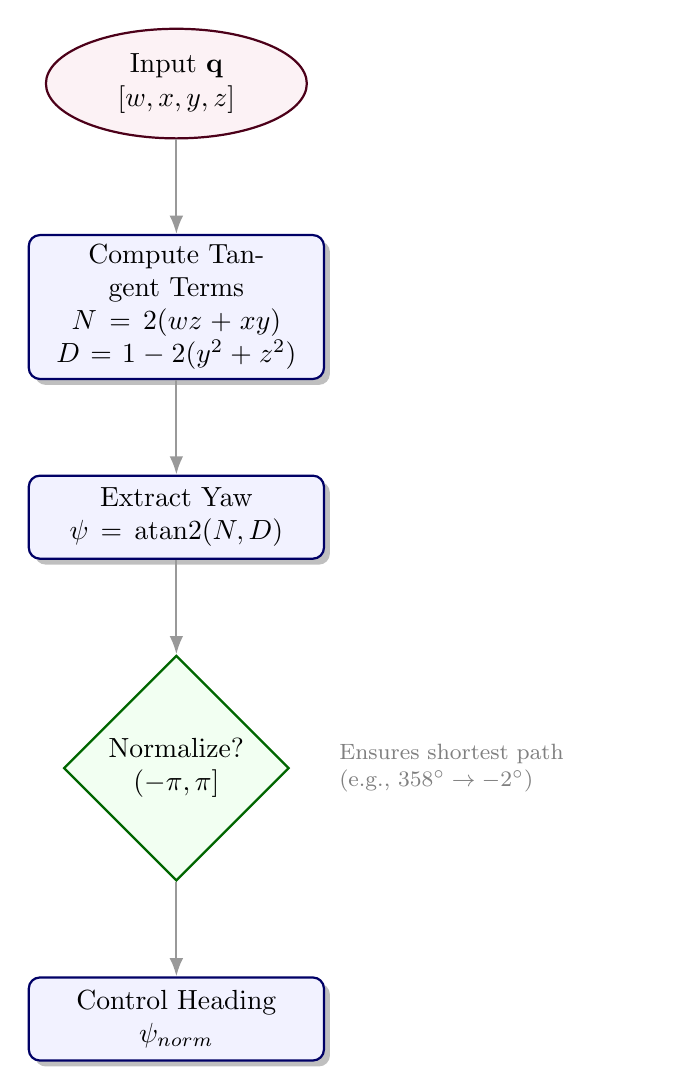
\begin{tikzpicture}[
        node distance=1.2cm,
        auto,
        block/.style={
            rectangle, 
            draw=blue!40!black, 
            thick, 
            fill=blue!5, 
            text width=10em, 
            align=center, 
            rounded corners, 
            minimum height=3em,
            drop shadow
        },
        input/.style={
            ellipse, 
            draw=purple!40!black, 
            thick, 
            fill=purple!5, 
            text width=6em, 
            align=center
        },
        decision/.style={
            diamond, 
            draw=green!40!black, 
            thick, 
            fill=green!5, 
            text width=6em, 
            align=center, 
            inner sep=0pt
        },
        line/.style={
            draw, 
            -Latex, 
            thick, 
            gray!80
        }
    ]
        % Nodes
        \node [input] (quat) {Input $\mathbf{q}$ \\ $[w, x, y, z]$};
        \node [block, below=of quat] (matrix) {Compute Tangent Terms \\ $N = 2(wz + xy)$ \\ $D = 1 - 2(y^2 + z^2)$};
        \node [block, below=of matrix] (atan) {Extract Yaw \\ $\psi = \text{atan2}(N, D)$};
        \node [decision, below=of atan] (norm) {Normalize? \\ $(-\pi, \pi]$};
        \node [block, below=of norm] (output) {Control Heading \\ $\psi_{norm}$};

        % Edges
        \draw [line] (quat) -- (matrix);
        \draw [line] (matrix) -- (atan);
        \draw [line] (atan) -- (norm);
        \draw [line] (norm) -- (output);
        
        % Annotation
        \node [right=0.5cm of norm, text width=4cm, font=\footnotesize, align=left, color=gray] {Ensures shortest path\\(e.g., $358^\circ \to -2^\circ$)};

    \end{tikzpicture}
    }
    \caption{Heading Extraction }
    \label{fig:quat_flow}
\end{figure}

\subsubsection{Euler Angles and the Singularity Problem}
Euler angles describe orientation as a sequence of three elemental rotations around body-fixed axes. For marine surface vessels, the standard Tait-Bryan $ZYX$ convention is employed:
\begin{itemize}
    \item \textbf{Yaw ($\psi$):} Rotation about the $z$-axis.
    \item \textbf{Pitch ($\theta$):} Rotation about the $y$-axis.
    \item \textbf{Roll ($\phi$):} Rotation about the $x$-axis.
\end{itemize}
However, Euler angle representations suffer from intrinsic singularities. If the Pitch angle $\theta$ approaches $\pm 90^\circ$, the Roll and Yaw axes become aligned (collinear), reducing the degrees of freedom to two. This condition, termed Gimbal Lock, causes the mathematical solution for orientation to become undefined or unstable.

\subsubsection{Unit Quaternions}
To mitigate this, the system utilizes Unit Quaternions  for robust state tracking. A quaternion $\mathbf{q}$ is a hyper-complex number system extending the complex plane into four dimensions:
\begin{equation}
    \mathbf{q} = q_w + q_x \mathbf{i} + q_y \mathbf{j} + q_z \mathbf{k}
\end{equation}
represented vectorially as $\mathbf{q} = [q_w, q_x, q_y, q_z]^T$, subject to the unit norm constraint $||\mathbf{q}|| = 1$. This representation provides a continuous, singularity-free mapping of the rotation group $SO(3)$.

\subsubsection{Derivation of Heading (Yaw)}
To extract the control-relevant Yaw angle $\psi$ from the quaternion, the quaternion is first mapped to the Direction Cosine Matrix (Rotation Matrix) $R_b^n(\mathbf{q})$. The general form of this matrix in terms of quaternion elements is given by:

\begin{equation}
    R_b^n(\mathbf{q}) = 
    \begin{bmatrix} 
    1 - 2(q_y^2 + q_z^2) & 2(q_x q_y - q_z q_w) & 2(q_x q_z + q_y q_w) \\
    2(q_x q_y + q_z q_w) & 1 - 2(q_x^2 + q_z^2) & 2(q_y q_z - q_x q_w) \\
    2(q_x q_z - q_y q_w) & 2(q_y q_z + q_x q_w) & 1 - 2(q_x^2 + q_y^2)
    \end{bmatrix}
\end{equation}

For a planar navigation problem where the primary variable of interest is the heading $\psi$, the relationship between the body-frame $x$-axis projected onto the inertial frame is examined. This corresponds to the matrix elements $R_{11}$ and $R_{21}$ (the first column of the rotation matrix), which relate to the tangent of the yaw angle:

\begin{equation}
    \tan(\psi) = \frac{R_{21}}{R_{11}} = \frac{2(q_w q_z + q_x q_y)}{1 - 2(q_y^2 + q_z^2)}
\end{equation}

By applying the four-quadrant inverse tangent function ($\text{atan2}$), the full heading angle is recovered in the range $(-\pi, \pi]$:
\begin{equation}
    \psi = \text{atan2}\left( 2(q_w q_z + q_x q_y), 1 - 2(q_y^2 + q_z^2) \right)
\end{equation}

\subsubsection{Domain Normalization}
The raw calculated angle may exceed standard bounds during continuous rotation (e.g., multiple full turns). For the PID controller to function correctly without "unwinding" behavior, the error signal is normalized to the shortest-path domain:
\begin{equation}
    \psi_{norm} = \text{atan2}(\sin(\psi), \cos(\psi))
\end{equation}
This ensures that a commanded turn from $179^\circ$ to $-179^\circ$ is treated as a $2^\circ$ right turn rather than a $358^\circ$ left turn.

\section{Mathematical Model Derivation}
The vessel's maneuvering dynamics are approximated using a phenomenological "black-box" model, specifically the First-Order Nomoto Model. This model abstracts the complex hydrodynamic interactions (added mass, damping, Coriolis forces) into two identifiable parameters: indices $K$ and $T$.

\subsection{Steering Dynamics (Yaw)}
The Nomoto model describes the transfer function between the rudder angle $\delta$ and the yaw rate $r$:
\begin{equation}
    \frac{r(s)}{\delta(s)} = \frac{K}{1 + Ts}
\end{equation}

In the time domain, this is expressed as the differential equation:
\begin{equation}
    T \dot{r} + r = K \delta
\end{equation}

Where:
\begin{itemize}
    \item $K \ [s^{-1}]$: The gain constant, representing the steady-state turning velocity per unit rudder angle.
    \item $T \ [s]$: The time constant, representing the vessel's inertial response lag.
\end{itemize}

\subsubsection{Non-Linear Parameter Variation}
To capture the non-linear hydrodynamic damping inherent in marine vessels, $K$ and $T$ are not static. The system implements a dynamic scheduling algorithm based on the rudder angle magnitude $|\delta|$:
\begin{align}
    K(\delta) &= K_{base} + K_{\delta} |\delta| \\
    T(\delta) &= T_{base} + T_{\delta} |\delta|
\end{align}
This allows the simulation to replicate the loss of turning efficiency at high rudder angles (stall regions) or varying hull characteristics.

\subsection{Surge Dynamics (Speed)}
Longitudinal motion is modeled as a first-order system with non-linear drag coupling. The surge acceleration $\dot{u}$ is derived from the balance of commanded thrust and hydrodynamic resistance:

\begin{equation}
    \dot{u} = \frac{1}{\tau_u} (u_{cmd} - u) - X_{added}(r)
\end{equation}

Where $X_{added}$ represents the added resistance due to maneuvering (speed bleed). Following standard steering equations (Norrbin, 1971), this is modeled as a non-linear damping term proportional to the square of the yaw rate:
\begin{equation}
    X_{added}(r) = C_d \cdot r^2
\end{equation}
This term ensures that the vessel realistically decelerates during turns regardless of direction, mimicking the increased hydrodynamic cross-section presented to the flow.

% =============================================================================
% CHAPTER 2.6: SENSOR SYSTEMS
% =============================================================================

\section{Sensor Systems and Signal Processing}
\label{sec:sensors}

The ASV Control Center utilizes a closed-loop feedback architecture driven by a suite of virtualized environmental sensors. To facilitate Software-in-the-Loop (SiL) validation, the system acts as both the \textit{generator} of sensor data (simulating physical hardware) and the \textit{processor} of that data (simulating the control computer).

\subsection{Communication Architecture}
The sensor interface is abstracted through the ROS 2 middleware. The communication topology follows a synchronous Publisher-Subscriber pattern operating at a deterministic frequency of 20Hz ($T_s = 50ms$).

\begin{figure}[H]
    \centering
    \includegraphics[width=1\linewidth]{top_topology.jpeg}
    \caption{Communication Topology}
    \label{fig:sensor_flow}
\end{figure}
As illustrated in Figure \ref{fig:sensor_flow}, the data flow is bidirectional:
\begin{enumerate}
    \item \textbf{Physics Layer:} The \texttt{Dynamics Node} solves the differential equations of motion and injects the resulting state vector into standard ROS message types.
    \item \textbf{Control Layer:} The navigation stack ingests these messages, applies signal conditioning, and computes the error signals for the PID controllers.
\end{enumerate}

\subsection{Global Navigation Satellite System (GNSS)}
Position tracking is managed by a virtualized GNSS receiver mimicking the behavior of a standard GPS module.

\subsubsection{Publisher Node}
The simulation module converts the local Cartesian position $(x, y)$ in meters into Geodetic coordinates (Latitude $\phi$, Longitude $\lambda$). The system employs an Equirectangular Projection model, assuming a local flat-earth approximation where longitudinal convergence is negligible for the operational range ($< 5km$).

The transformation used by the publisher on the \texttt{gps} topic is:
\begin{align}
    \phi_{sim}(t) &= \phi_{ref} + \left( \frac{y(t)}{R_{scale}} \right) \\
    \lambda_{sim}(t) &= \lambda_{ref} + \left( \frac{x(t)}{R_{scale}} \right)
\end{align}
In the provided implementation, the uniform scaling factor $R_{scale}$ is linearized to a constant $111,139 \text{ m/deg}$, representing the average meridional radius of curvature.



\subsubsection{Receiver Node}
The control node subscribes to the GNSS topic. To utilize this data for velocity control, the system must differentiate the positional stream to recover the velocity vector.

\textbf{1. Coordinate Re-projection:}
The incoming Geodetic stream is projected back to the local Tangent Plane using the inverse of the simulation scaling:
\begin{equation}
    x_{meas} = (\lambda_{meas} - \lambda_{ref}) \cdot 111139.0
\end{equation}
\begin{equation}
    y_{meas} = (\phi_{meas} - \phi_{ref}) \cdot 111139.0
\end{equation}

\textbf{2. Velocity Estimation (Finite Difference):}
Since standard consumer GPS units often output position at a lower rate than the control loop, the system derives the linear velocity vector $\mathbf{v}_{lin}$ using a First-Order Backwards Difference method:
\begin{equation}
    \mathbf{v}_{lin}[k] = \frac{\mathbf{p}_{meas}[k] - \mathbf{p}_{meas}[k-1]}{\Delta t}
\end{equation}
Where $\mathbf{p}_{meas} = [x_{meas}, y_{meas}]^T$. This derived velocity serves as the process variable (PV) for the Surge Speed PID controller.

\begin{figure}[H]
    \centering
    \resizebox{\linewidth}{!}{
    \begin{tikzpicture}[
        % Grid layout for perfect alignment
        node distance=1.5cm and 1cm,
        % --- Defined Styles ---
        % 1. Physics & Actuator (The Physical World)
        phys_block/.style={
            rectangle, rounded corners=3pt,
            draw=blue!40!black, thick,
            top color=white, bottom color=blue!10,
            minimum width=3.5cm, minimum height=1.5cm,
            align=center, font=\bfseries\small,
            drop shadow
        },
        % 2. The ROS Topic (Communication)
        topic_block/.style={
            rectangle, chamfered corners,
            draw=orange!80!black, thick,
            fill=orange!5, dashed,
            minimum width=3cm, minimum height=1cm,
            align=center, font=\footnotesize\ttfamily
        },
        % 3. The Computing Blocks (Processing & Control)
        logic_block/.style={
            rectangle, rounded corners=3pt,
            draw=green!40!black, thick,
            top color=white, bottom color=green!10,
            minimum width=3.5cm, minimum height=1.5cm,
            align=center, font=\bfseries\small,
            drop shadow
        },
        % 4. Connection Lines
        flow_line/.style={
            ->, >={Latex[length=3mm, width=2mm]},
            draw=gray!70!black, line width=1.2pt,
            rounded corners=5pt, font=\scriptsize\sffamily
        }
    ]

        % --- ROW 1: SENSOR DATA FLOW (Left to Right) ---
        
        % Node 1: Physics
        \node[phys_block] (physics) {\\ Physics Engine\\ \normalfont\footnotesize (State: $x,y$)\\};
        
        % Node 2: GPS Topic
        \node[topic_block, right=of physics] (topic) {GPS\\ \normalfont\scriptsize (NavSatFix)};
        
        % Node 3: Signal Processing
        \node[logic_block, right=of topic] (process) {Control Node\\ \normalfont\footnotesize (Coordinate Re-projection\\ \normalfont\footnotesize\&\\ \normalfont\footnotesize Velocity Estimation)};

        % --- ROW 2: CONTROL FEEDBACK FLOW (Right to Left) ---
        
        % Node 4: PID Controller (Placed below Processing)
        \node[logic_block, below=of process, draw=red!40!black, bottom color=red!10] (pid) {Speed PID\\ \normalfont\footnotesize };
        
        % Node 5: Actuator Interface (Placed below Physics)
        \node[phys_block, below=of physics, draw=gray!80!black, bottom color=gray!10] (actuator) {\\Actuator\\ };

        % --- CONNECTIONS ---

        % 1. Physics -> Topic
        \draw[flow_line] (physics) -- node[above] {Encode } (topic);
        
        % 2. Topic -> Processing
        \draw[flow_line] (topic) -- node[above] {Decode } (process);
        
        % 3. Processing -> PID (Vertical Down)
        \draw[flow_line] (process) -- node[right] {Measured Velocity} (pid);
        
        % 4. PID -> Actuator (Horizontal Return)
        \draw[flow_line] (pid) -- node[above] {Command Thrust ($u_{cmd}$)} (actuator);
        
        % 5. Actuator -> Physics (Vertical Up - Closing the Loop)
        \draw[flow_line] (actuator) -- node[left] {Update State} (physics);

        % --- Background Container for Context ---
        \begin{scope}[on background layer]
            \node[draw=gray!20, dashed, fill=gray!5, inner sep=0.5cm, fit=(physics) (process) (actuator) (pid), rounded corners=10pt] {};
        \end{scope}

    \end{tikzpicture}
    }
    \caption{GNSS Control Topology: A structured view of the closed-loop architecture. The upper layer handles the sensor simulation pipeline (Physics $\to$ Encoding $\to$ Decoding $\to$ Velocity Estimation). The lower layer handles the control response (PID $\to$ Thrust Command $\to$ Physics Update).}
    \label{fig:gps_topology_clean}
\end{figure}

\subsection{Inertial Measurement Unit (IMU)}
The vessel is equipped with a virtual 6-axis MEMS IMU, providing high-frequency updates on angular rates and linear accelerations. To facilitate robust state estimation, the simulator models a "Strapdown" inertial system attached to the vessel's Center of Gravity (CG).

\subsubsection{Publisher Node (Virtualization)}
The physics engine synthesizes IMU telemetry by transforming the calculated body-frame kinematics into proper acceleration and angular rates.

\textbf{1. Angular Velocity (Gyroscope):}
The gyroscope output $\boldsymbol{\omega}_{gyro}$ correlates directly to the vessel's body-fixed rotational rates. While the simulator calculates full 3D orientation for visualization, the control logic focuses on the planar Yaw Rate ($r$), yielding the simplified output vector:
\begin{equation}
    \boldsymbol{\omega}_{gyro} = \begin{bmatrix} p \\ q \\ r \end{bmatrix} \approx \begin{bmatrix} 0 \\ 0 \\ r \end{bmatrix}
\end{equation}

\textbf{2. Linear Acceleration (Accelerometer):}
The accelerometer measures "Proper Acceleration" ($\mathbf{f}^b$), which is the vector sum of kinematic acceleration, Coriolis/Centripetal terms, and the reaction to gravity. The general strapdown equation is:
\begin{equation}
    \mathbf{f}^b = \dot{\mathbf{v}}^b + (\boldsymbol{\omega}^b \times \mathbf{v}^b) - \mathbf{R}_n^b \mathbf{g}^n
\end{equation}

In the specific implementation, system assumes small roll/pitch angles and planar motion ($v \approx 0, w \approx 0$), this simplifies to the calculation used in the physics kernel:
\begin{equation}
    \mathbf{a}_{sim} = \begin{bmatrix}
    \dot{u} \\
    u \cdot r \\
    g
    \end{bmatrix}
\end{equation}
\textbf{Note:} The term $u \cdot r$ represents the centripetal acceleration experienced during a turn. Including this term is used for preventing "drift" in state estimators that rely on inertial integration, as it accounts for the rotating reference frame of the turning vessel.


\subsubsection{Receiver Node}
The control system ingests the raw IMU message to derive higher-order derivative states required for advanced model-based control.

\textbf{Angular Acceleration Derivation:}
Standard IMUs provide angular velocity $\boldsymbol{\omega}$, but not angular acceleration. To anticipate inertial lags in the vessel's response (specifically the $T$ parameter in Nomoto models), the system estimates the angular acceleration vector $\boldsymbol{\alpha}$ using a First-Order Backwards Difference method:
\begin{equation}
    \boldsymbol{\alpha}[k] = \frac{\boldsymbol{\omega}_{meas}[k] - \boldsymbol{\omega}_{meas}[k-1]}{\Delta t}
\end{equation}
This derivative term quantifies the rotational energy change, serving as a input for the "Update Physics" observer which validates the dynamic Nomoto parameters in real-time.

\begin{figure}[H]
    \centering
    \resizebox{\linewidth}{!}{
    \begin{tikzpicture}[
        node distance=2cm and 2cm,
        % --- Styles ---
        phys_block/.style={
            rectangle, rounded corners=3pt,
            draw=blue!40!black, thick,
            top color=white, bottom color=blue!10,
            minimum width=4cm, minimum height=1.8cm,
            text width=3.5cm,
            align=center, font=\bfseries\small,
            drop shadow
        },
        topic_block/.style={
            rectangle, chamfered corners,
            draw=orange!80!black, thick,
            fill=orange!5, dashed,
            minimum width=4cm, minimum height=1.2cm,
            text width=3.5cm,
            align=center, font=\footnotesize\ttfamily
        },
        logic_block/.style={
            rectangle, rounded corners=3pt,
            draw=green!40!black, thick,
            top color=white, bottom color=green!10,
            minimum width=4cm, minimum height=1.8cm,
            text width=3.5cm,
            align=center, font=\bfseries\small,
            drop shadow
        },
        obs_block/.style={
            logic_block, draw=purple!40!black, bottom color=purple!10
        },
        flow_line/.style={
            ->, >={Latex[length=3mm, width=2mm]},
            draw=gray!70!black, line width=1.2pt,
            rounded corners=5pt, font=\scriptsize\sffamily
        }
    ]

        % --- Nodes ---
        % Top Row
        \node[phys_block] (physics) {Physics Engine\\ \normalfont\footnotesize (Kinematics: $\dot{u}, u, r$)};
        \node[topic_block, right=of physics] (topic) {IMU};
        
        % Bottom Row
        \node[logic_block, below=of topic] (diff) {Differentiation\\ \normalfont\footnotesize $\alpha = \Delta \omega / \Delta t$};
        \node[obs_block, left=of diff] (observer) {Inertial Observer\\ };

        % --- Connections ---
        % 1. Physics -> Topic
        \draw[flow_line] (physics) -- node[above] {Synthesize Data} (topic);
        
        % 2. Topic -> Diff
        \draw[flow_line] (topic) -- node[right] {Subscribe} (diff);
        
        % 3. Diff -> Observer
        \draw[flow_line] (diff) -- node[above] {Angular Accel} (observer);
        
        % 4. Validation (Dashed Upward)
        \draw[flow_line, dashed] (observer) -- node[left] {Validation} (physics);

        % --- Background ---
        \begin{scope}[on background layer]
            \node[draw=gray!20, dashed, fill=gray!5, inner sep=0.5cm, fit=(physics) (topic) (diff) (observer), rounded corners=10pt] {};
        \end{scope}

    \end{tikzpicture}
    }
    \caption{IMU Signal Topology: The Physics Engine computes proper acceleration. The Control Node differentiates gyroscope data to recover angular acceleration ($\alpha$) for the observer.}
    \label{fig:imu_topology}
\end{figure}

\subsection{Rudder Actuation Feedback}
The steering system utilizes a virtual absolute encoder to provide closed-loop feedback for the heading controller, ensuring that the simulated physics engine and the control logic remain synchronized.

\subsubsection{Data Structure}
The actuator state is broadcast via the standard ROS 2 \texttt{ joint states} topic. The message contains the raw angular displacement of the rudder stock $\delta$, encoded in radians to adhere to SI standards.

\subsubsection{Signal Processing}
Upon receipt, the raw encoder signal undergoes normalization and conditioning before being utilized by the hydrodynamic solver.

\textbf{1. Unit Conversion:}
To facilitate operator interpretation and consistent parameter scheduling, the radian input is converted to degrees:
\begin{equation}
    \delta_{deg} = \delta_{rad} \cdot \left( \frac{180}{\pi} \right)
\end{equation}

\textbf{2. Limit Clamping (Mechanical Stops):}
To simulate physical steering constraints, the control logic saturates the input command to the vessel's effective rudder range. This prevents integral windup in the PID controller and ensures the Nomoto model operates within valid linearization bounds:
\begin{equation}
    \delta_{eff} = \text{sat}(\delta_{raw}, \delta_{lim}) = \begin{cases} 
      \delta_{lim} & \text{if } \delta_{raw} > \delta_{lim} \\
      -\delta_{lim} & \text{if } \delta_{raw} < -\delta_{lim} \\
      \delta_{raw} & \text{otherwise}
   \end{cases}
\end{equation}
This effective angle $\delta_{eff}$ serves as the direct input to the variable Nomoto gain $K(\delta)$ and time constant $T(\delta)$ scheduling functions described in Section 2.3.

\begin{figure}[H]
    \centering
    \resizebox{\linewidth}{!}{
    \begin{tikzpicture}[
        node distance=2cm and 2cm,
        % --- Styles ---
        box/.style={
            rectangle, rounded corners=3pt,
            draw=blue!40!black, thick, 
            fill=blue!5, 
            minimum width=3.0cm, minimum height=1.5cm,
            align=center, font=\bfseries\small,
            drop shadow
        },
        topic/.style={
            rectangle, chamfered corners,
            draw=orange!80!black, thick, 
            fill=orange!5, dashed, 
            minimum width=3.5cm, minimum height=1cm,
            align=center, font=\footnotesize\ttfamily
        },
        logic/.style={
            box, draw=green!40!black, fill=green!5
        },
        line/.style={
            ->, >={Latex[length=3mm, width=2mm]},
            draw=gray!70!black, line width=1.2pt,
            rounded corners=5pt, font=\scriptsize\sffamily
        }
    ]

        % --- Nodes ---
        \node[box] (phys) {Physics Engine\\ \normalfont\footnotesize (Nomoto State $\delta$)};
        \node[topic, right=of phys] (topic) {joint states};
        \node[logic, right=of topic] (proc) {Unit Conversion\\ \normalfont\footnotesize (Rad $\to$ Deg)};
        \node[box, below=of proc, draw=red!40!black, fill=red!5] (sched) {Parameter Scheduling\\ \normalfont\footnotesize Update $K(\delta), T(\delta)$};

        % --- Connections ---
        \draw[line] (phys) -- node[above] {Encoder Read} (topic);
        \draw[line] (topic) -- node[above] {Subscribe} (proc);
        \draw[line] (proc) -- node[right] {$\delta_{deg}$} (sched);
        \draw[line] (sched) -- node[above] {Update Coeffs} (sched -| phys) -- (phys);

        % --- Container ---
        \begin{scope}[on background layer]
            \node[draw=gray!20, dashed, fill=gray!5, inner sep=0.5cm, fit=(phys) (topic) (proc) (sched), rounded corners=10pt] {};
        \end{scope}

    \end{tikzpicture}
    }
    \caption{Rudder Feedback Topology: The closed-loop cycle where actuator state determines the hydrodynamic coefficients ($K, T$) for the next physics step.}
    \label{fig:rudder_topology}
\end{figure}

\subsection{Data Synchronization and Fusion}
The ASV Control Center functions within a distributed ROS 2 architecture where sensor telemetry and actuator feedback arrive asynchronously. To maintain temporal coherence between the physics engine and the control logic, the system abstracts the asynchronous message passing into a Synchronous Sampled-Data System.

\subsubsection{Deterministic Event Loop}
Synchronization is enforced via a centralized Application Loop driven by a high-precision timer, rather than relying on non-deterministic ROS callbacks. Operating at a fixed frequency of $f_s = 20\text{Hz}$, this architecture ensures that simulation time advances linearly with wall-clock time, effectively decoupling the physics solver from network jitter.

\subsubsection{The Control Cycle}
In each discrete time-step $k$, the system executes a strict sequence of atomic operations to close the feedback loop:

\begin{enumerate}
    \item \textbf{Data Ingestion (Spin):} The system explicitly triggers the ROS executor (spin once) to digest all pending messages in the subscriber queue.
    
    \item \textbf{Zero-Order Hold (ZOH) Fusion:} 
    Since sensors publish at different rates, the state estimator applies a Zero-Order Hold strategy. The internal state vector $\mathbf{x}[k]$ is updated using the \textit{most recent} buffered values from the GNSS and IMU topics. If a sensor packet is delayed, the system holds the value from $\mathbf{x}[k-1]$, ensuring the solver never blocks waiting for data.
    
    \item \textbf{Control Law Update:} 
    The PID algorithms compute the required control efforts (Thrust $u_{cmd}$ and Rudder $\delta_{cmd}$) based on the synchronized state snapshot $\mathbf{x}[k]$.
    
    \item \textbf{Physics Integration:} 
    Finally, the Nomoto solver advances the vessel's kinematic state for the interval $[t, t + \Delta t]$ using the computed control inputs, guaranteeing a deterministic time-step ($dt = 0.05s$) for the numerical integration.
\end{enumerate}
% =============================================================================
% CHAPTER 3: CONTROL SYSTEM DESIGN
% =============================================================================

\section{Control System Design}
\label{sec:control_system}

The ASV control architecture is designed to manage two primary DoF: Surge Speed and Heading. The system operates in three distinct selectable control modes allowing for flexible testing of both open-loop actuation and closed-loop autonomy.

\subsection{Control Architecture Overview}
The system implements a cascaded decision logic where the active source of control signals is determined by the selected mode. \\\\\\\\\\\\\\\\\\

\begin{figure}[H]
    \centering
    \resizebox{\linewidth}{!}{
    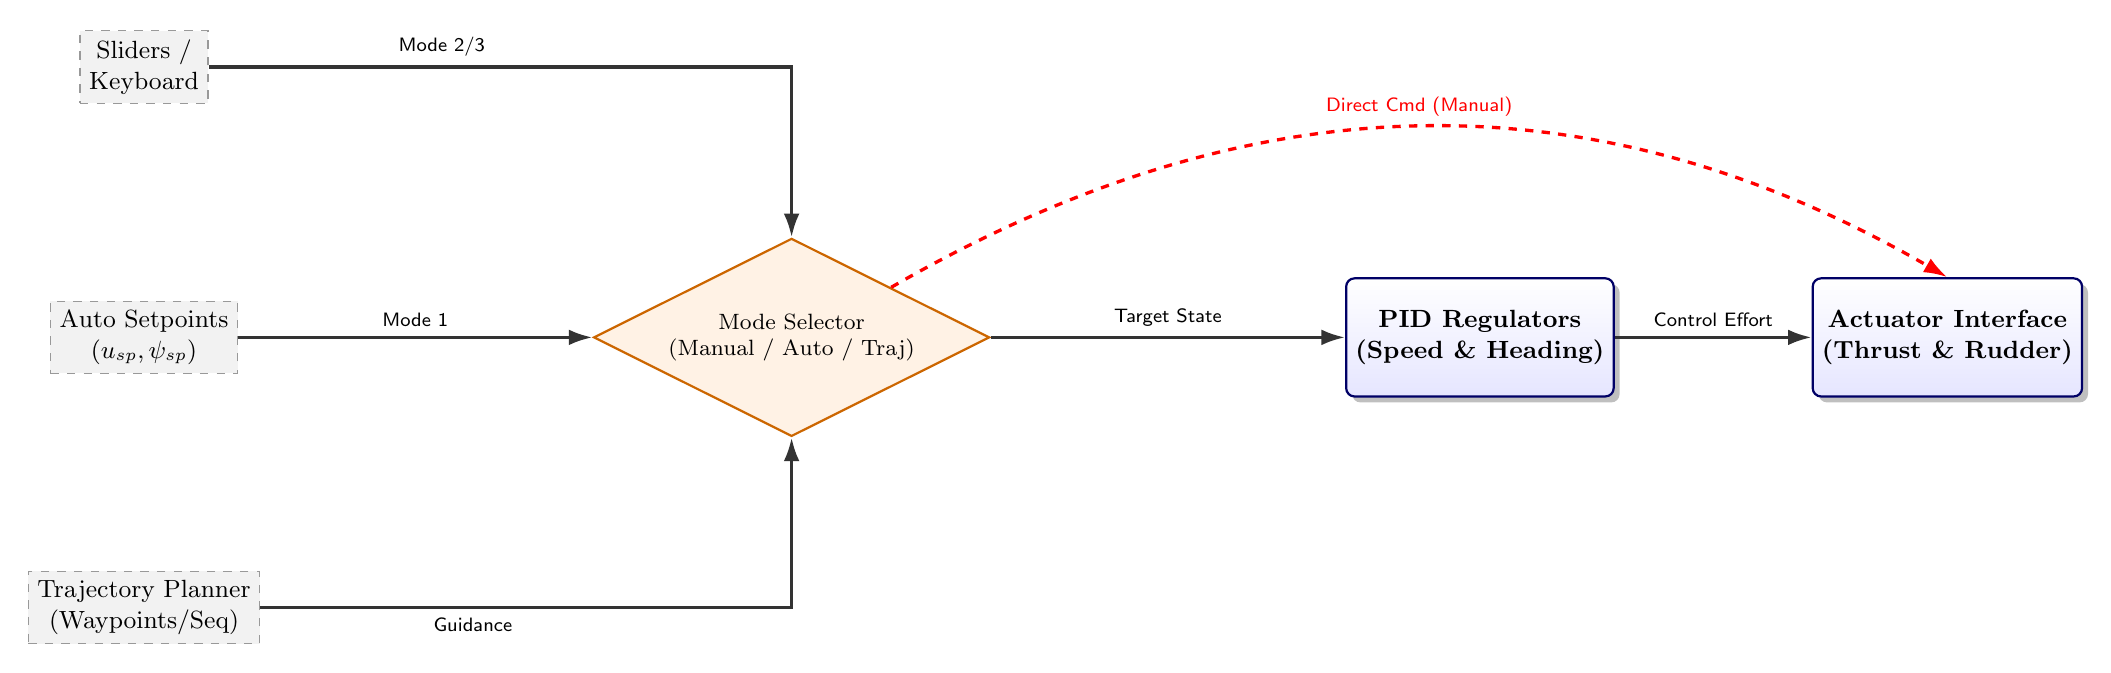
\begin{tikzpicture}[
        node distance=2.5cm and 2.5cm,
        % Styles
        block/.style={
            rectangle, rounded corners=3pt,
            draw=blue!40!black, thick,
            top color=white, bottom color=blue!10,
            minimum width=3cm, minimum height=1.5cm,
            align=center, font=\bfseries\small,
            drop shadow
        },
        decision/.style={
            diamond, aspect=2,
            draw=orange!80!black, thick,
            fill=orange!10,
            minimum width=3cm,
            align=center, font=\footnotesize
        },
        input/.style={
            rectangle, draw=gray!80, fill=gray!10, dashed, align=center, font=\small
        },
        line/.style={
            ->, >={Latex[length=3mm, width=2mm]},
            draw=black!80, line width=1.2pt, font=\scriptsize\sffamily
        }
    ]

        % Inputs
        \node[input] (gui_man) {Sliders /\\Keyboard};
        \node[input, below=of gui_man] (gui_sp) {Auto Setpoints\\($u_{sp}, \psi_{sp}$)};
        \node[input, below=of gui_sp] (traj) {Trajectory Planner\\(Waypoints/Seq)};

        % Switch
        \node[decision, right=of gui_sp, xshift=2cm] (switch) {Mode Selector\\(Manual / Auto / Traj)};

        % Controllers
        \node[block, right=of switch, xshift=2cm] (pid) {PID Regulators\\(Speed \& Heading)};
        
        % Plant
        \node[block, right=of pid] (plant) {Actuator Interface\\(Thrust \& Rudder)};

        % Connections
        \draw[line] (gui_man) -| node[pos=0.2, above] {Mode 2/3} (switch.north);
        \draw[line] (gui_sp) -- node[above] {Mode 1} (switch.west);
        \draw[line] (traj) -| node[pos=0.2, below] {Guidance} (switch.south);

        % Switch Outputs
        \draw[line] (switch.east) -- node[above] {Target State} (pid.west);
        
        % PID to Plant
        \draw[line] (pid.east) -- node[above] {Control Effort} (plant.west);
        
        % Manual Bypass (Visual Only - logic handles this internally)
        \draw[line, dashed, color=red] (switch.north east) to[out=30, in=150] node[above, color=red] {Direct Cmd (Manual)} (plant.north);

    \end{tikzpicture}
    }
    \caption{Control System Architecture: The central switching logic routes either raw operator commands (Manual) or PID-computed efforts (Auto/Trajectory) to the vessel actuators.}
    \label{fig:control_arch}
\end{figure}

\subsection{Manual Control Modes}
Manual operation allows operators to inject open-loop signals directly into the physics engine, bypassing the PID regulators.

\subsubsection{Slider Control (Direct)}
In "Slider Mode," the GUI widgets map directly to the actuator limits. The command vector $\mathbf{u}_{cmd}$ is derived as:
\begin{align}
    u_{cmd}(t) &= \frac{\text{Slider}_u}{100} \cdot V_{max} \\
    \delta_{cmd}(t) &= \text{Slider}_r \quad [\text{deg}]
\end{align}
where $V_{max} = 5.0$ m/s. This provides a "Step Input" capability for analyzing transient response.

\subsubsection{Keyboard Control (Teleoperation)}
In "Arrow Mode," the system implements a dynamic accumulator with auto-centering decay, mimicking a physical joystick's return-to-center behavior.
\begin{itemize}
    \item \textbf{Acceleration:} When a key is held, the command increments by $\alpha = 0.2$.
    \item \textbf{Decay:} When released, the command decays towards zero by $\beta = 0.1$.
\end{itemize}
The discrete update law implemented in the event loop is:
\begin{equation}
    u[k] = \begin{cases} 
    u[k-1] + \alpha & \text{if Key}_{\uparrow} \\
    u[k-1] - \alpha & \text{if Key}_{\downarrow} \\
    u[k-1] - \text{sgn}(u[k-1]) \cdot \beta & \text{else (Decay)}
    \end{cases}
\end{equation}
A similar logic applies to the rudder with an increment of $1.5^\circ$ and a strong centering decay ($2.0^\circ$) to simulate hydrodynamic realignment.

\subsection{Automatic Control (PID)}
In "Auto Mode," the system activates two independent PID controllers to regulate Speed and Heading. The controllers operate on the error signal calculated at $20\text{Hz}$.

\subsubsection{Speed Controller}
The surge velocity is regulated by a standard PID acting on the error $e_u[k] = u_{sp} - u_{meas}[k]$.
\begin{equation}
    u_{out} = K_p e_u + K_i \sum e_u \Delta t + K_d \frac{e_u - e_{u,prev}}{\Delta t}
\end{equation}
To prevent integrator windup during saturation (e.g., full throttle), the integral term $I$ is clamped. The final output is saturated to the vessel's speed limits.

\subsubsection{Heading Controller}
Heading control requires special handling of the angular domain to avoid discontinuity at $\pm 180^\circ$. The error is normalized to the shortest path:
\begin{equation}
    e_{\psi} = \text{atan2}(\sin(\psi_{sp} - \psi_{meas}), \cos(\psi_{sp} - \psi_{meas}))
\end{equation}
The PID output is inverted (negative feedback) to drive the rudder angle $\delta$:
\begin{equation}
    \delta_{cmd} = -1.0 \cdot \left( K_p e_{\psi} + K_d \frac{e_{\psi} - e_{\psi,prev}}{\Delta t} \right)
\end{equation}
\textit{Note:} The derivative term is computed on the error, which effectively provides rate damping ($K_d \dot{e} \approx -K_d r$) assuming a constant setpoint.

\section{Trajectory and Mission Planning}
The system includes a high-level guidance layer capable of executing waypoint-based paths and pre-programmed rudder sequences.

\begin{figure}[H]
    \centering
    \resizebox{0.9\linewidth}{!}{
    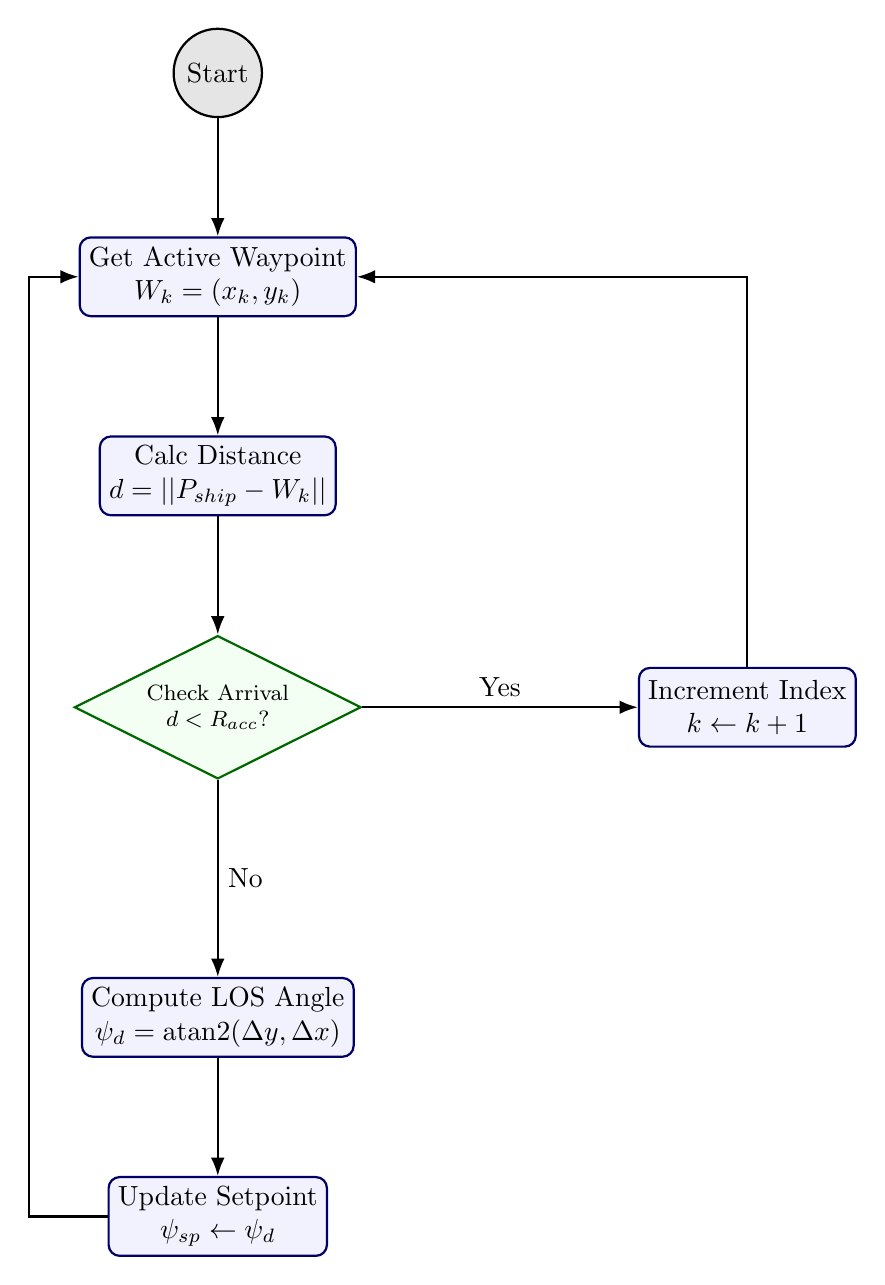
\begin{tikzpicture}[
        node distance=1.5cm and 1.5cm,
        start/.style={circle, draw=black, fill=gray!20, thick, minimum size=1cm},
        process/.style={rectangle, draw=blue!40!black, fill=blue!5, thick, rounded corners, minimum height=1cm, align=center},
        decision/.style={diamond, aspect=2, draw=green!40!black, fill=green!5, thick, align=center, font=\footnotesize},
        arrow/.style={-Latex, thick}
    ]

        \node[start] (start) {Start};
        \node[process, below=of start] (get_wp) {Get Active Waypoint\\$W_k = (x_k, y_k)$};
        \node[process, below=of get_wp] (calc_dist) {Calc Distance\\$d = ||P_{ship} - W_k||$};
        \node[decision, below=of calc_dist] (check) {Check Arrival\\$d < R_{acc}$?};
        
        \node[process, right=of check, xshift=2cm] (switch) {Increment Index\\$k \leftarrow k+1$};
        \node[process, below=of check, yshift=-1cm] (los) {Compute LOS Angle\\$\psi_d = \text{atan2}(\Delta y, \Delta x)$};
        \node[process, below=of los] (send) {Update Setpoint\\$\psi_{sp} \leftarrow \psi_d$};

        \draw[arrow] (start) -- (get_wp);
        \draw[arrow] (get_wp) -- (calc_dist);
        \draw[arrow] (calc_dist) -- (check);
        
        \draw[arrow] (check.east) -- node[above] {Yes} (switch);
        \draw[arrow] (switch.north) |- (get_wp.east);
        
        \draw[arrow] (check.south) -- node[right] {No} (los);
        \draw[arrow] (los) -- (send);
        \draw[arrow] (send.west) -- ++(-1,0) |- (get_wp.west);

    \end{tikzpicture}
    }
    \caption{The Line-of-Sight (LOS) guidance loop }
    \label{fig:traj_logic}
\end{figure}

\subsection{Path Planner }
Autonomous navigation utilizes a Line-of-Sight (LOS) guidance law. The planner decomposes a global path defined by a list of coordinate tuples $W = \{w_0, w_1, ..., w_n\}$.

\subsubsection{Guidance Law}
For the active target waypoint $w_k = (x_k, y_k)$, the desired heading $\psi_d$ is computed geometrically relative to the vessel's current position $(x, y)$:
\begin{equation}
    \psi_d(t) = \text{atan2}(y_k - y(t), x_k - x(t))
\end{equation}
This desired heading is fed directly into the Heading PID controller ($\psi_{sp} = \psi_d$).

\subsubsection{Waypoint Switching Logic}
To ensure smooth path transitions, the sequencer monitors the Euclidean distance $d(t)$ to the target. A "Sphere of Acceptance" criterion triggers the switching event:
\begin{equation}
    \text{Trigger}(k \to k+1) \iff \sqrt{(x_k - x)^2 + (y_k - y)^2} < R_{acc}
\end{equation}
In the current implementation, the acceptance radius is set to $R_{acc} = 1.0$ meter.

\subsection{Rudder Sequence Scheduler}
For validating hydrodynamic parameters, the system can execute a deterministic "Rudder Schedule" (e.g., Zig-Zag maneuvers). This mode bypasses the heading PID and injects timed open-loop commands.

The sequence is defined as a queue of tuples $Q = \{( \delta_0, t_0 ), ( \delta_1, t_1 ), ... \}$. A dedicated timer executes the queue:
\begin{equation}
    \delta_{cmd}(t) = \delta_i \quad \text{for} \quad t_{start,i} \le t < t_{start,i} + t_i
\end{equation}


% =============================================================================
% CHAPTER 4: USER INTERFACE AND OPERATION
% =============================================================================

\section{Software Initialization}
Upon launching the application, the user is greeted by the Splash Screen (Figure \ref{fig:splash}). This landing page performs background checks on the ROS 2 middleware connectivity.

\begin{figure}[H]
    \centering
    \includegraphics[width=1\linewidth]{home_screen.png}
    \caption{Application Entry Point: The ASV Sim Splash Screen allows the user to initialize the simulation kernel or access documentation before entering the main control loop.}
    \label{fig:splash}
\end{figure}

Selecting “Run Simulation” initializes the backend services and opens the main operational interface. The Documentation button provides access to the technical documentation. If Skip Guide is not enabled, the basic helper guide is automatically launched. The Exit buttons terminate the application.

\section{Main Dashboard Overview}
The core interface is designed for situational awareness. As shown in Figure \ref{fig:main_gui}, the "Current Status" panel at the top-left provides a numerical readout of the vessel's state vector.\\\\

\begin{figure}[H]
    \centering
    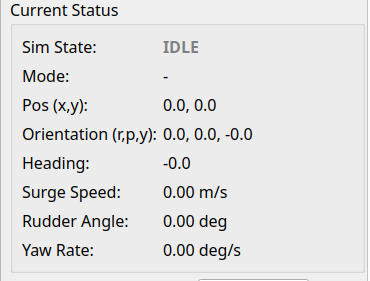
\includegraphics[width=0.5\linewidth]{current_stat.png}
    \caption{The Current Status Panel}
    \label{fig:main_gui}
\end{figure}

\textbf{Status Indicators:}
\begin{itemize}
    \item \textbf{Sim State:} Indicates if the physics engine is integrating (`RUNNING`), frozen (`PAUSED`) or Resets all it states to initial conditions and waiting for re-initiation (`IDLE`).
    \item  \textbf{Mode:} Showing the active control mode
    \item \textbf{Pos (x,y):} Global position in meters relative to the start origin.
    \item \textbf{Orientation (r,p,y): } Orientations (roll, pitch, yaw) in degrees
    \item \textbf{Heading:} The vessel's current Yaw angle ($\psi$) in degrees.
    \item \textbf{Surge Speed:} Forward velocity ($u$) in m/s.
    \item \textbf{Rudder Angle: } Current in command rudder angle in degrees
    \item \textbf{Yaw Rate: } Measured instantaneous yaw ratw value
\end{itemize}

\section{Simulation Lifecycle Management}
Located at the top-left of the Control Sidebar (Figure \ref{fig:sim_ctrl}), the Simulation Control group manages the execution state of the physics kernel.

\begin{figure}[H]
    \centering
    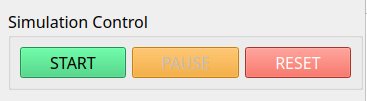
\includegraphics[width=0.6\linewidth]{global_cont_top.png}
    \caption{Global Simulation Controls}
    \label{fig:sim_ctrl}
\end{figure}

The interface provides three distinct states:
\begin{itemize}
    \item \textbf{START :} Engages the application timer. This triggers the loop callback at 20Hz, enabling real-time physics integration, sensor publishing, and controller execution.
    \item \textbf{PAUSE :} Freezes the simulation time $t$. The vessel's kinematic state vector $\mathbf{x}(t)$ is preserved in memory, allowing the operator to inspect instantaneous values without the system drifting.
    \item \textbf{RESET :} Performs a "Hard Reset". This action:
    \begin{enumerate}
        \item Zeros the state vector (Position $x=0, y=0$, Heading $\psi=0$).
        \item Flushes the PID integrator buffers (preventing "integral windup" from previous runs).
        \item Resets the simulation clock to $t=0.0s$.
    \end{enumerate}
\end{itemize}

\section{Control Modes}
The "Controls" tab allows the operator to select the active input source. The system supports three distinct modes of operation.

\subsection{Manual Control (Sliders \& Keyboard)}
For open-loop testing and step-response analysis, the \textbf{Manual (Sliders)} mode is used. This connects the GUI widgets directly to the simulated actuators.

\begin{figure}[H]
    \centering
    % --- Left Figure ---
    \begin{minipage}[t]{0.48\linewidth}
        \centering
        % Note: You used the same image file for both. Update filename if needed.
        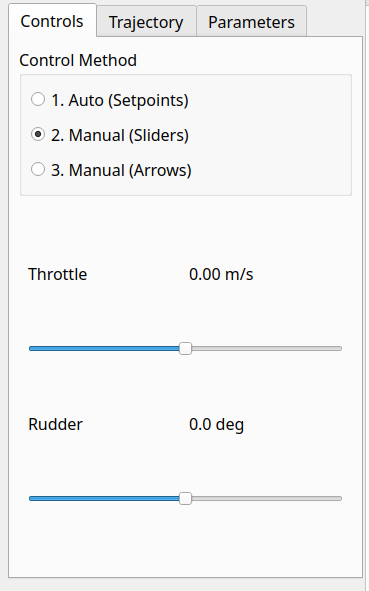
\includegraphics[width=\linewidth]{control_method_sl.png}
        \caption{Manual Control (Slider).}
        \label{fig:manual_ctrl_slider} % Note: Changed label to be unique
    \end{minipage}
    \hfill % Adds horizontal space between figures
    % --- Right Figure ---
    \begin{minipage}[t]{0.48\linewidth}
        \centering
        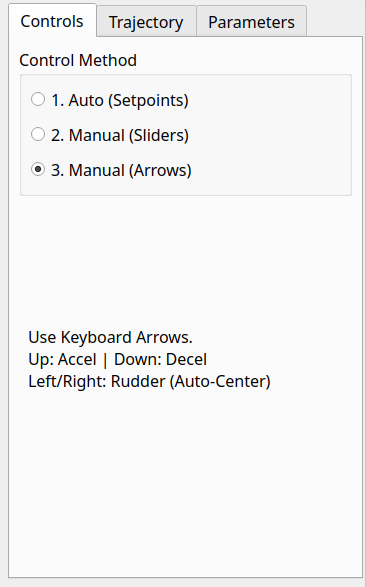
\includegraphics[width=\linewidth]{control_method_arrow.png}
        \caption{Manual Control (Arrows).}
        \label{fig:manual_ctrl_arrows} % Note: Changed label to be unique
    \end{minipage}
\end{figure}

\begin{itemize}
    \item \textbf{Throttle Slider:} Sets the target surge speed ($u_{cmd}$) between $-5.0$ and $+5.0$ m/s.
    \item \textbf{Rudder Slider:} Sets the rudder angle ($\delta_{cmd}$) within the mechanical limits of $\pm 17^\circ$.
    \item \textbf{Keyboard Shortcuts:} In "Arrow Mode," the Up/Down keys increment throttle, while Left/Right keys actuate the rudder with an auto-centering decay to simulate a joystick.
\end{itemize}

\section{Trajectory and Mission Planning}
The "Trajectory" tab switches the system to autonomous guidance. This interface allows users to design paths or schedule deterministic maneuver sequences.

\subsection{Waypoint Navigation}
The Waypoint Planner (Figure \ref{fig:traj_wp}) enables Point-to-Point navigation using the Line-of-Sight (LOS) guidance law. 

\begin{figure}[H]
    \centering
    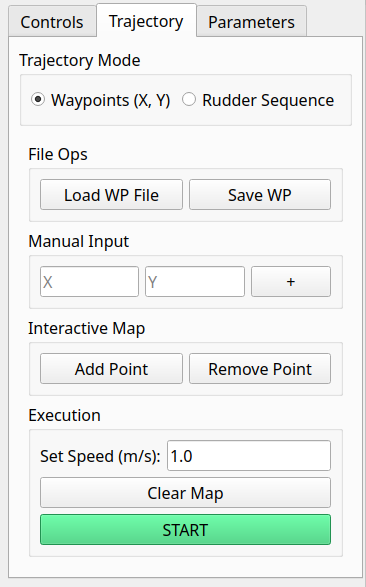
\includegraphics[width=0.45\linewidth]{trajectory_wp.png}
    \caption{Trajectory Planner Panel.}
    \label{fig:traj_wp}
\end{figure}

\textbf{Operational Features:}
\begin{itemize}
    \item \textbf{Interactive Map:} When "Add Point" is toggled, clicking anywhere on the 2D grid (Right Panel) appends a coordinate to the mission queue. In order to remove one-by-one "Remove Point" options must be used. Clear map option clear all the points at once.
    \item \textbf{File Ops:} Standard `.txt` files containing `x,y` coordinates can be loaded via browsing with 'Load WP File' button for repeatable mission profiles v. If the edited map is wanted to preserve for later use 'Save WP' will open a folder browser for user to select where to save waypoints file (same format as load wp file).
    \item \textbf{Execution:} Setting the "Set Speed" and clicking \textbf{START} engages the Autopilot. The vessel will autonomously navigate the waypoints in sequence.
\end{itemize}

\subsection{Rudder Sequence Scheduler}
For hydrodynamic parameter identification (e.g., Zig-Zag tests), the Rudder Sequence mode (Figure \ref{fig:traj_seq}) is used. This bypasses the heading controller to execute a timed queue of open-loop commands.

\begin{figure}[H]
    \centering
    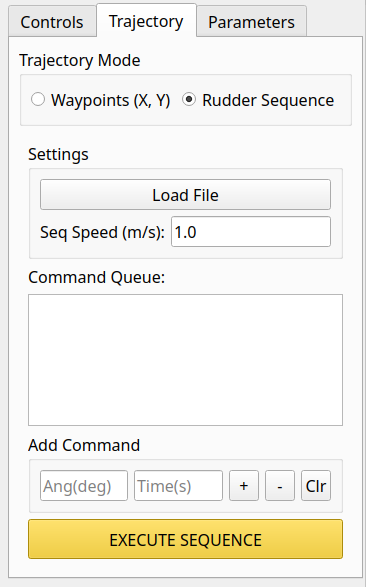
\includegraphics[width=0.45\linewidth]{trajectory_rudder.png}
    \caption{Rudder Sequence Scheduler Panel}
    \label{fig:traj_seq}
\end{figure}

\textbf{Operational Features:}
\begin{itemize}
    \item \textbf{Global Sequence Speed:} Before defining the turns, the user sets a constant surge velocity (e.g., $2.0$ m/s) in the "Seq Speed" field. This ensures the vessel maintains sufficient kinetic energy throughout the maneuver.
    \item \textbf{Command Queue Construction:} The user can either load pre-determined rudder schedule from 'Load File' or can build the mission profile iteratively. By entering a specific Rudder Angle (degrees) and Duration (seconds) and clicking the \textbf{`+`} button, the tuple is added to the "Command Queue" list widget (e.g., "Rudder: $15^\circ$ for $5.0$s").
    \item \textbf{Queue Management:} The interface provides tools for error correction; the \textbf{`-`} button removes the selected command, while the \textbf{`Clr`} button purges the entire schedule.
    \item \textbf{Real-Time Execution:} Clicking \textbf{EXECUTE SEQUENCE} (Yellow Button) engages the mission timer. The system automatically highlights the currently active command in the list view as it progresses, providing the operator with immediate visual feedback on the maneuver's stage.
\end{itemize}

\section{Parameter Tuning}
The "Parameters" tab (Figure \ref{fig:params}) provides a direct interface to the physics engine's internal coefficients.

\begin{figure}[H]
    \centering
    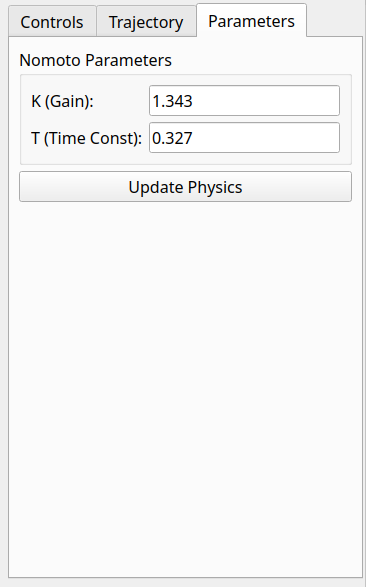
\includegraphics[width=0.45\linewidth]{params.png}
    \caption{Real-Time Parameter Injection Panel}
    \label{fig:params}
\end{figure}

This feature enables the application to be used with different types of marine vessels, rather than being limited to a single vessel type.

\section{Real-Time Visualization}
The Right Panel is dedicated to high-fidelity data visualization, essential for analyzing system performance.

\subsection{Time-Series Plots}
Three stacked graphs display the history of the last 25 seconds (500 samples):
\begin{figure}[H]
    \centering
    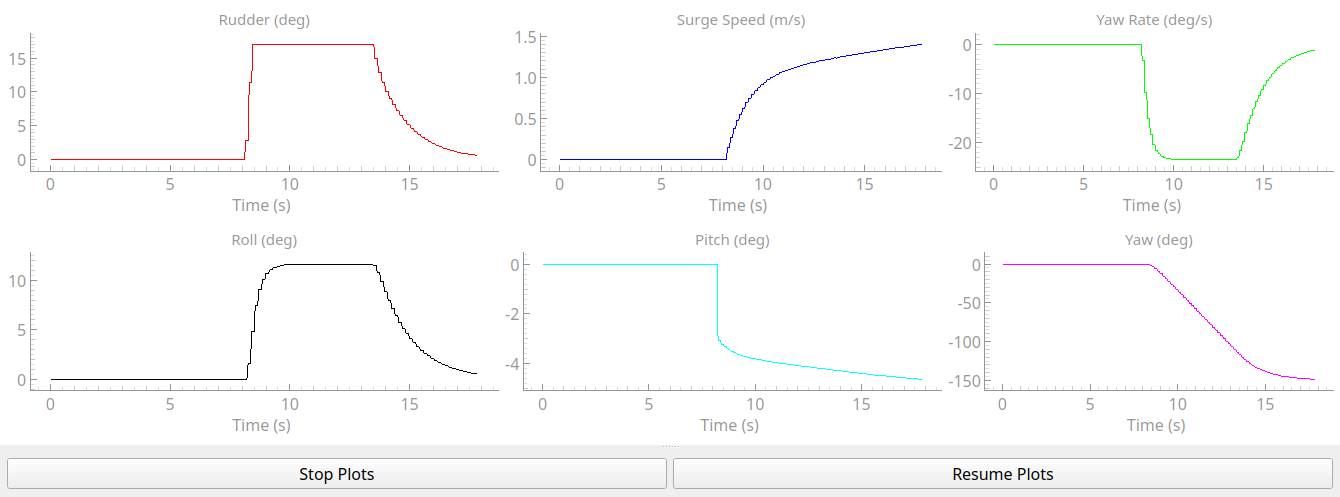
\includegraphics[width=1\linewidth]{plot_panel.png}
    \caption{Time-Series Plots}
\end{figure}

\subsection{2D Trajectory Map}
The bottom grid creates a spatial "God's Eye View" of the simulation.
\begin{figure}[H]
    \centering
    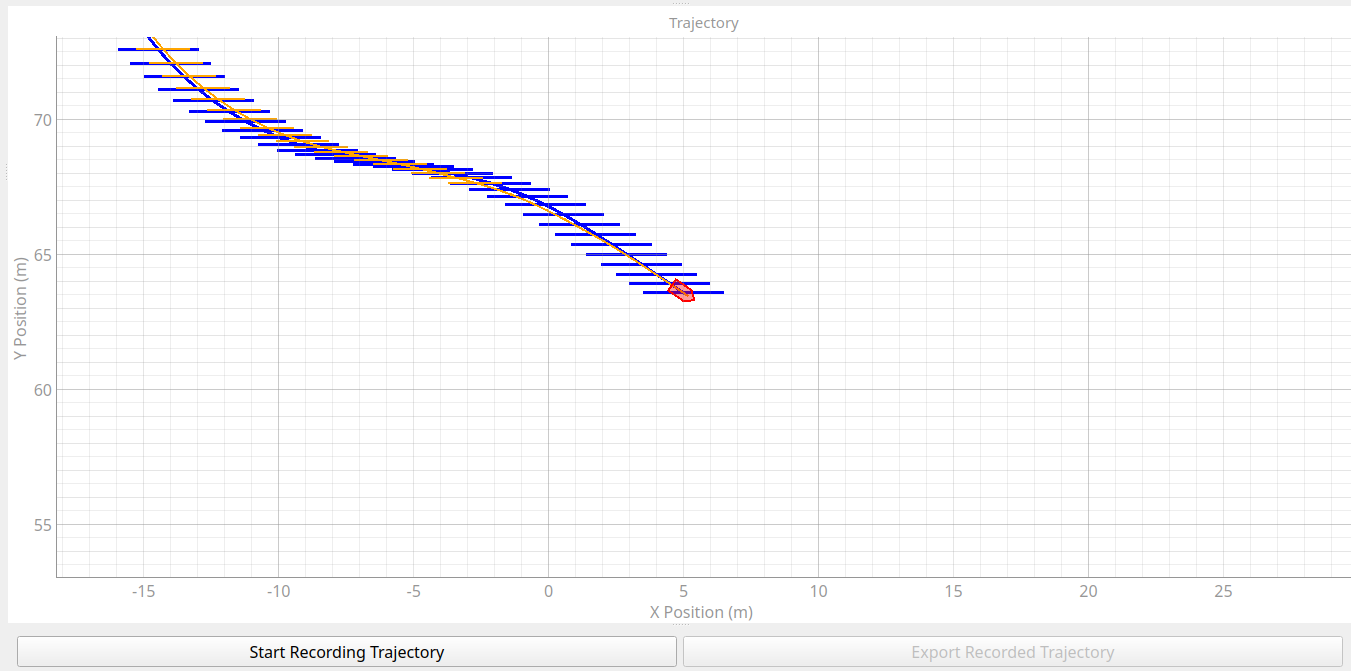
\includegraphics[width=1\linewidth]{trajectory_panel.png}
    \caption{Trajectory Panel}
\end{figure}
\begin{itemize}
    \item \textbf{Blue Trace:} The vessel's actual path.
    \item \textbf{Orange Trace:} The "Nomoto Prediction" path (ideal model).
    \item \textbf{Red Dashed Line:} The active Waypoint path (if in Trajectory mode).
    \item \textbf{Vessel Icon:} A red polygon representing the ship's current position and orientation ($\psi$).
\end{itemize}

Beneath the trajectory panel, two buttons are provided for video trajectory recording. Selecting Start Recording Trajectory opens a folder selection dialog, allowing the user to choose the destination directory. From that point onward, video recording begins and is continuously written to the selected location until the user selects Export Recording Trajectory, which finalizes the recording.

\section{Data Logging and Export}
For post-mission analysis, the ASV Control Suite includes a built-in telemetry recorder located at the bottom of the sidebar (Figure \ref{fig:data_log}).

\begin{figure}[H]
    \centering
    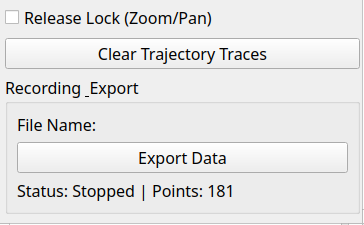
\includegraphics[width=0.6\linewidth]{global_cont_bottom.png}
    \caption{Data Recording Interface: Tools for managing the visual workspace and exporting high-fidelity simulation data for external analysis.}
    \label{fig:data_log}
\end{figure}

\subsection{Visual Trace Management}
During long-duration simulations, the 2D map can become cluttered with overlapping path history.
\begin{itemize}
    \item \textbf{Release Lock:} By checking "Release Lock (Zoom/Pan)," the user decouples the camera from the vessel, allowing free exploration of the map using the mouse wheel and drag gestures.
    \item \textbf{Clear Trajectory Traces:} Clicking this button wipes the visual history (Blue/Orange lines) from the plotting widget \textit{without} resetting the physics engine. This is useful for clearing the screen between repetitive maneuvers.
\end{itemize}

\subsection{Telemetry Export}
The system automatically buffers all sensor data and internal state variables into a RAM history queue while the simulation is \texttt{RUNNING}.

\textbf{Export Workflow:}
\begin{enumerate}
    \item \textbf{Suspend Simulation:} It is recommended to transition the simulation state to \texttt{PAUSED} before exporting. This freezes the data buffer, ensuring that the exported dataset represents a complete and consistent time-slice without write conflicts.
    \item \textbf{Initiate Export:} Clicking the \textbf{"Export Data"} button invokes the operating system's native file dialog, allowing the user to define the destination path.
    \item \textbf{Format Selection:} The system supports saving data in either \texttt{.csv} (Comma Separated Values) for universal compatibility or \texttt{.xlsx} (Microsoft Excel) for immediate spreadsheet analysis.
\end{enumerate}

\noindent The exported telemetry file is structured with high-precision floating-point values, organized into the following column groups:
\begin{itemize}
    \item \textbf{Temporal Data:} Simulation elapsed time ($t_{sim}$) and the corresponding Real-world UTC timestamp for log synchronization.
    \item \textbf{Navigational State:} Global Cartesian coordinates ($x, y$) and the normalized Heading angle ($\psi$).
    \item \textbf{Vessel Dynamics:} Surge Velocity ($u$), Yaw Rate ($r$), and estimated Euler attitudes for Roll ($\phi$) and Pitch ($\theta$).
    \item \textbf{Actuator Feedback:} The instantaneous Rudder Angle ($\delta$) and active Throttle commands.
\end{itemize}




\end{document}